
\section{Planning Language}\label{S:PDDL}
The Planning Domain Definition Language (PDDL) \cite{PDDL} is an attempt by the domain independent planning community to formulate a standard language for planning. A community of planning researchers has been producing planning systems that comply with this formalism since the first International Planning Competition held in 1998. This competition series
continues today, with the seventh competition being held in 2011. PDDL is constantly adding extensions to the base language in order to represent more expressive problem domains. Our work is based on PDDL Version 3.\\
By placing our knowledge in a PDDL representation, we enable the use of an entire family of open source planning systems.
Each PDDL file-set consists of two files that specify the domain and the problem.

\subsection{The PDDL Domain File}\label{S:PDDL-domain}
The PDDL domain file for kitting is consists of five sections that include \texttt{requirements}, \texttt{types}, \texttt{predicates}, \texttt{functions}, and \texttt{actions}. An excerpt of the PDDL domain file is depicted in Figure~\ref{fig:domain}.

\begin{figure}[t!h!]
\begin{minipage}{.5\paperwidth}
\begin{mylisting}
\begin{Verbatim}[commandchars=\\\{\},fontsize=\scriptsize, numbers=left, numbersep=2pt]
(define (domain kitting-domain)
    (:requirements :strips :typing :fluents)
    (:types EndEffector EndEffectorHolder Kit KitTray LargeBoxWithEmptyKitTrays 
        PartsTray EndEffectorChangingStation Robot WorkTable LargeBoxWithKits Part)

    (:predicates
	   (endeffector-location-robot ?endeffector - EndEffector ?robot - Robot)	
	   (on-worktable-kit ?worktable - WorkTable ?kit - Kit))

    (:functions
	   (quantity-partstray ?partstray - PartsTray)
	   (quantity-kit ?kit - Kit ?partstray - PartsTray)
	   (capacity-kit ?kit - Kit ?partstray - PartsTray))

    (:action take-kittray
        :parameters(
            ?robot - Robot
            ?kittray - KitTray
            ?largeboxwithemptykittrays - LargeBoxWithEmptyKitTrays
            ?endeffector - EndEffector
            ?worktable - WorkTable)
        :precondition(and
            (robot-empty ?robot)
            (lbwekt-not-empty ?largeboxwithemptykittrays)
            (robot-with-endeffector ?robot ?endeffector)
            (kittray-location-lbwekt ?kittray ?largeboxwithemptykittrays)
            (endeffector-location-robot ?endeffector ?robot)
            (worktable-empty ?worktable)
            (endeffector-type-kittray ?endeffector ?kittray))
        :effect(and
            (robot-holds-kittray ?robot ?kittray)
            (kittray-location-robot ?kittray ?robot)
            (not (robot-empty ?robot))
            (not (kittray-location-lbwekt ?kittray ?largeboxwithemptykittrays))))
)

\end{Verbatim}
\end{mylisting}
\end{minipage}
\caption{Excerpt of the PDDL domain file for kitting.}
\label{fig:domain}
\end{figure}

\begin{itemize}
\item line 1: The keyword \texttt{domain} signals a planner that this file contains information on the domain. \texttt{kitting-domain} is the name given to the domain.
\item line 2: The \texttt{:requirements} field specifies which section the domain relies on. The planning system can examine this statement to determine if it is capable of solving problems in this domain. A keyword (symbol starting with a colon) used in a \texttt{:requirements} field is called a requirement flag; the domain is said to declare a requirement for that flag. The requirement flags present in the kitting domain are:
\begin{itemize}
\item \texttt{:strips}: The most basic subset of PDDL, consisting of STRIPS only.
\item \texttt{:typing}: PDDL has a special syntax for declaring parameter and object types. \texttt{:typing} allows types names in declaration of variables.
\item \texttt{:fluents}: A domain's set of requirements allow a planner to quickly tell if it is likely to be able
to handle the domain. For example, this version of the kitting world requires fluents numeric, so a straight STRIPS-representation planner would not be able to handle it. A fluent is a term (\texttt{:functions}) with time-varying value (i.e., a value that can change as a result of performing an action).
\end{itemize}
\item lines 3--4:  Type names have to be declared before they are used (before \texttt{:predicates} and \texttt{:functions}). This is done with the declaration \texttt{(:types $name_1$ ... $name_n$)}.
\item lines 6--8: The \texttt{:predicates} part of a domain definition specify only what are the predicate names used in the domain, and their number of arguments (and argument types, if the domain uses \texttt{:typing}). The ``meaning'' of a predicate, in the sense of for what combinations of arguments it can be true and its relationship to other predicates, is determined by the effects that actions in the domain can have on the predicate, and by what instances of the predicate are listed as true in the initial state of the problem definition.\\
    It is common to make a distinction between static and dynamic predicates. A \textit{static} predicate is not changed by any action. Thus in a problem, the true and false instances of a \textit{static} predicate will always be precisely those listed in the initial state specification of the problem definition. Note that there is no syntactic difference between \textit{static} and \textit{dynamic} predicates in PDDL, they look exactly the same in the \texttt{:predicates} declaration part of the domain.\\
    A predicate is build using the structure \texttt{(predicate\_name ?X - type\_of\_X)}. A list of parameters of the same type in a predicate can be abbreviated to \texttt{(predicate\_name ?X ?Y ?Z - type\_of\_XYZ)}. Note that the hyphen between parameter and type name is surrounded by whitespace.
\item lines 10--13: A fluent is similar to a state variable/predicate except that its value is a number instead of true or false. The initial value of a function is set in the initial state of the problem file and changes when an action is executed. The declaration of functions is similar to predicates.
\item lines 15--34: The domain definition contains operators (called \textit{actions} in PDDL). An action statement specifies a way that a planner affects the state of the world. The statement includes parameters, preconditions, and effects. All parts of an action definition except the name are, according to the PDDL specification, optional (although, of course, an action without effects is pretty useless). However, for an action that has no preconditions some planners may require an ``empty'' precondition, on the form :precondition () or :precondition (and), and some planners may also require an empty :parameter list for actions without parameters).
\begin{itemize}
\item lines 16--21: The \texttt{:parameters} section declare all the parameters used by predicates and functions in \texttt{preconditions} and \texttt{effects}.
\item lines 22--29: The \texttt{:preconditions} section is a conjunction of predicates and functions that need to be true in the world in order for the action to be invoked.
\item lines 30--34: The \texttt{:effects} equation dictates the changes in the world that will occur due to the execution of the action.
\end{itemize}
\end{itemize}


\subsection{PDDL Problem File}\label{S:PDDL-problem}
The second file of the PDDL file-set is a  problem file. The problem file specifies information about the specific instance of the given problem. This file contains the initial conditions and definition of the world (in the \texttt{init} section) and the final state that the world must be brought to (in the \texttt{goal} section). Using an example of kit to build, this section only describes the initial and goal states explicitly. The operators detailed in Section~\ref{subsect:Planning_Operators} are used by a planner to generate the other states as needed.\\
In the PDDL problem file depicted below, the \class{Robot} has to build a kit that contains two \class{Parts} of type A, one \class{Part} of type B and one \class{Part} of type C. The kitting process is completed once the \class{Kit} is placed in the \class{LargeBoxWithKits}.

\begin{center}
\begin{minipage}{.9\paperwidth}
\begin{mylisting}
\begin{Verbatim}[commandchars=\\\{\},fontsize=\scriptsize, numbers=left, numbersep=2pt]
(define (problem kitting-problem)
    (:domain kitting-domain)
    (:objects
        robot_1 - Robot
        changing_station_1 - EndEffectorChangingStation
        kit_tray_1 - KitTray
        kit_a2b1c1 - Kit
        empty_kit_tray_supply - LargeBoxWithEmptyKitTrays
        finished_kit_receiver - LargeBoxWithKits
        work_table_1 - WorkTable
        part_a_tray part_b_tray part_c_tray - PartsTray
        part_a_1 part_a_2  - Part
        part_b_1 part_b_2 part_b_3 - Part
        part_c_1 part_c_2 - Part
        part_gripper tray_gripper - EndEffector
        part_gripper_holder tray_gripper_holder - EndEffectorHolder
    )
)
(:init
    (robot-with-no-endeffector robot_1)
    (part-not-searched)
    (lbwekt-not-empty empty_kit_tray_supply)	
    (lbwk-not-full finished_kit_receiver)		
    (partstray-not-empty part_a_tray)
    (partstray-not-empty part_b_tray)
    (partstray-not-empty part_c_tray)
    (endeffector-location-endeffectorholder part_gripper part_gripper_holder)
    (endeffector-location-endeffectorholder tray_gripper tray_gripper_holder)
    (endeffectorholder-holds-endeffector part_gripper_holder part_gripper)
    (endeffectorholder-holds-endeffector tray_gripper_holder tray_gripper)
    (endeffectorholder-location tray_gripper_holder changing_station_1)
    (endeffectorholder-location part_gripper_holder changing_station_1)
    (endeffectorchangingstation-contains-endeffectorholder changing_station_1 tray_gripper_holder)	
    (endeffectorchangingstation-contains-endeffectorholder changing_station_1 part_gripper_holder)
    (worktable-empty work_table_1)
    (kittray-location-lbwekt kit_tray_1 empty_kit_tray_supply)

\end{Verbatim}
\end{mylisting}
\end{minipage}

\begin{minipage}{.5\paperwidth}
\begin{mylisting}
\begin{Verbatim}[commandchars=\\\{\},fontsize=\scriptsize,  firstnumber=continue, numbers=left, numbersep=2pt]	

    (part-location-partstray part_a_1 part_a_tray)
    (part-location-partstray part_a_2 part_a_tray)
    (part-location-partstray part_b_1 part_b_tray)
    (part-location-partstray part_b_2 part_b_tray)
    (part-location-partstray part_b_3 part_b_tray)
    (part-location-partstray part_c_1 part_c_tray)
    (part-location-partstray part_c_2 part_c_tray)
	
    (endeffector-type-part part_gripper part_a_1)
    (endeffector-type-part part_gripper part_a_2)
    (endeffector-type-part part_gripper part_b_1)
    (endeffector-type-part part_gripper part_b_2)
    (endeffector-type-part part_gripper part_b_3)
    (endeffector-type-part part_gripper part_c_1)
    (endeffector-type-part part_gripper part_c_2)

    (endeffector-type-kittray tray_gripper kit_tray_1)
    (endeffector-type-kit tray_gripper kit_a2b1c1)

    (= (capacity-kit kit_a2b1c1 part_a_tray) 2)
    (= (capacity-kit kit_a2b1c1 part_b_tray) 1)
    (= (capacity-kit kit_a2b1c1 part_c_tray) 1)

    (= (quantity-kit kit_a2b1c1 part_a_tray) 0)
    (= (quantity-kit kit_a2b1c1 part_b_tray) 0)
    (= (quantity-kit kit_a2b1c1 part_c_tray) 0)
\end{Verbatim}
\end{mylisting}
\end{minipage}

\begin{minipage}{.5\paperwidth}
\begin{mylisting}
\begin{Verbatim}[commandchars=\\\{\},fontsize=\scriptsize,  firstnumber=continue, numbers=left, numbersep=2pt]	
    (= (quantity-partstray part_a_tray) 2)
    (= (quantity-partstray part_b_tray) 3)
    (= (quantity-partstray part_c_tray) 2)

    (origin-part part_a_1 part_a_tray)
    (origin-part part_a_2 part_a_tray)
    (origin-part part_b_1 part_b_tray)
    (origin-part part_b_2 part_b_tray)
    (origin-part part_b_3 part_b_tray)
    (origin-part part_c_1 part_c_tray)
    (origin-part part_c_2 part_c_tray)
)

(:goal
    (and
        (= (quantity-kit kit_a2b1c1 part_a_tray)(capacity-kit kit_a2b1c1 part_a_tray))
        (= (quantity-kit kit_a2b1c1 part_b_tray)(capacity-kit kit_a2b1c1 part_b_tray))
        (= (quantity-kit kit_a2b1c1 part_c_tray)(capacity-kit kit_a2b1c1 part_c_tray))
        (kit-location-lbwk kit_a2b2c1 finished_kit_receiver)
    )
)
\end{Verbatim}
\end{mylisting}
\end{minipage}
\end{center}

\begin{itemize}
\item line 1: Signal a planner that the file contains all the element part of a problem. \texttt{kitting-problem} is the name given to this problem.
\item line 2: \texttt{:domain} refers to the domain that the current problem is associated to. In this case, the problem refers to the domain \texttt{kitting-domain}. Note that \texttt{kitting-domain} is the name given to the kitting domain as presented in section~\ref{S:PDDL-domain}.
\item line 3--17: \texttt{:objects} declare objects present in the problem instance. The syntax for \texttt{:objects} is \texttt{$object_1$ - Type ... $object_n$ - Type}.
\end{itemize}
%\caption{The init section.}
%\label{fig:init}
%\end{figure}

\subsubsection{Initial State}
The initial state $S_0$ (Figure~\ref{fig:s0}) defines the environment in its initial condition. The initial state of the kitting problem in PDDL format is described below.

\begin{figure}[h!t!]
\centering
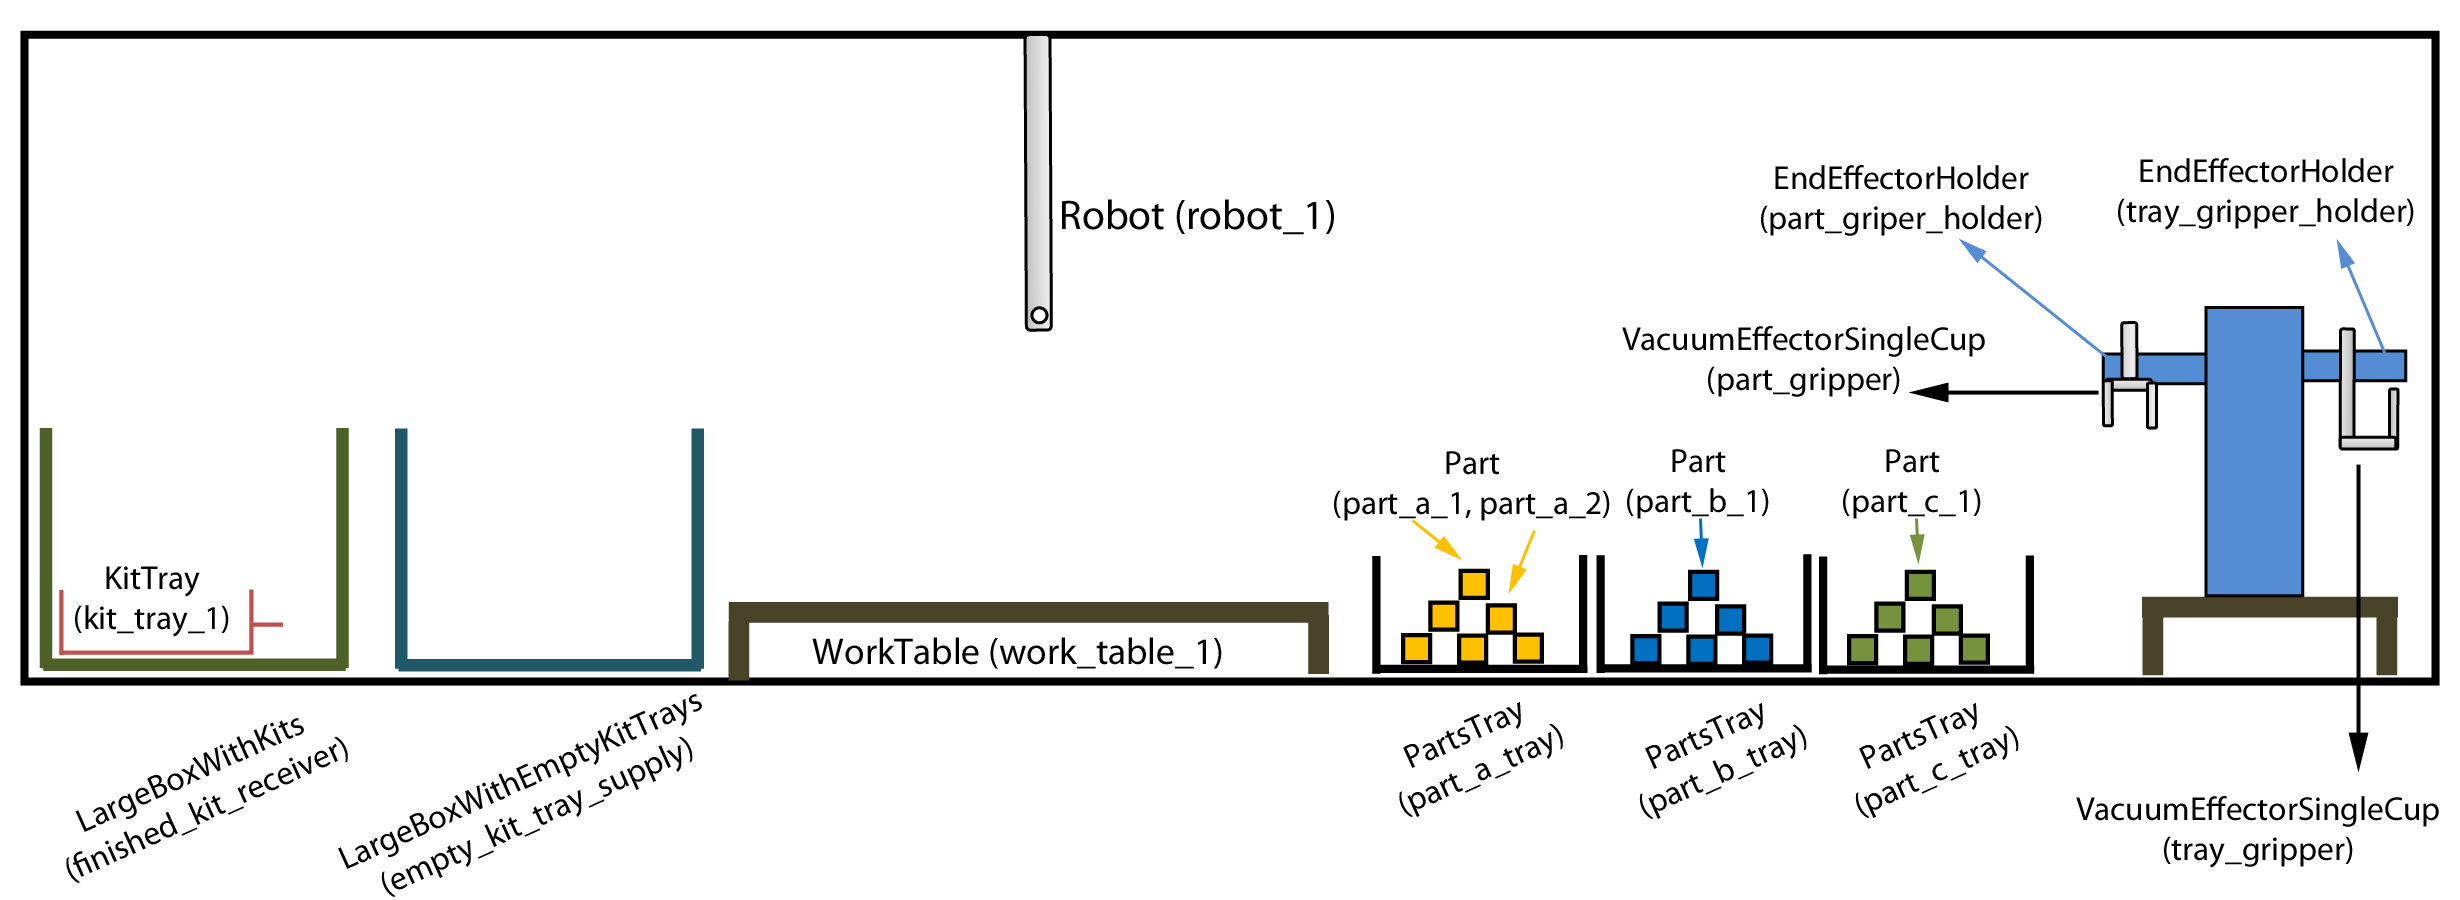
\includegraphics[width=14cm]{Figure/s0.jpg}
\caption{Initial state $S_0$.}
\label{fig:s0}
\end{figure}

\begin{itemize}
\item line 19: \texttt{:init} signals a planner that the predicates and functions in this section are true in the initial state.
\item line 20--76: Predicates true in the initial state of the environment. Since PDDL uses a close world assumption, predicates that are not present in the initial state are automatically set to false. This section also set the initial values for functions. Some relevant sections are presented:
\begin{itemize}
\item line 21: The predicate \stvarsmall{part-not-searched} is set to true so that the operator \op{look-for-part} can be activated during a plan search.
\item line 58--60: Functions describing how many parts of a specific type that \constsmall{kit\_a2b1c1} can contain. In this example, \constsmall{kit\_a2b1c1} can have two \class{Parts} of type A (\constsmall{part\_a\_tray}), one \class{Part} of type B (\constsmall{part\_b\_tray}), and one \class{Part} of type C (\constsmall{part\_c\_tray}).
\item line 62--64: Functions that represent the number of parts of a specific type that are already in \constsmall{kit\_a2b1c1}. In the initial state, \constsmall{kit\_a2b1c1} is empty (no \class{Parts} of type A, B, or C).
\item line 65--67: Functions that describe the number of parts available in their respective parts tray. This also can be read as: \emph{In the workstation, there are two \class{Parts} of type A available, three \class{Parts} of type B available, and three \class{Parts} of type C available}.
\item line 69--75: Predicates that describe the type of each specific part in the workstation. Defining that \texttt{part\_a\_1} is from \texttt{part\_a\_tray} is similar to \texttt{part\_a\_tray} is of type A since a \class{PartsTray} consists of parts of the same type.
\end{itemize}
\end{itemize}

\subsubsection{Goal State}
\begin{figure}[h!t!]
\centering
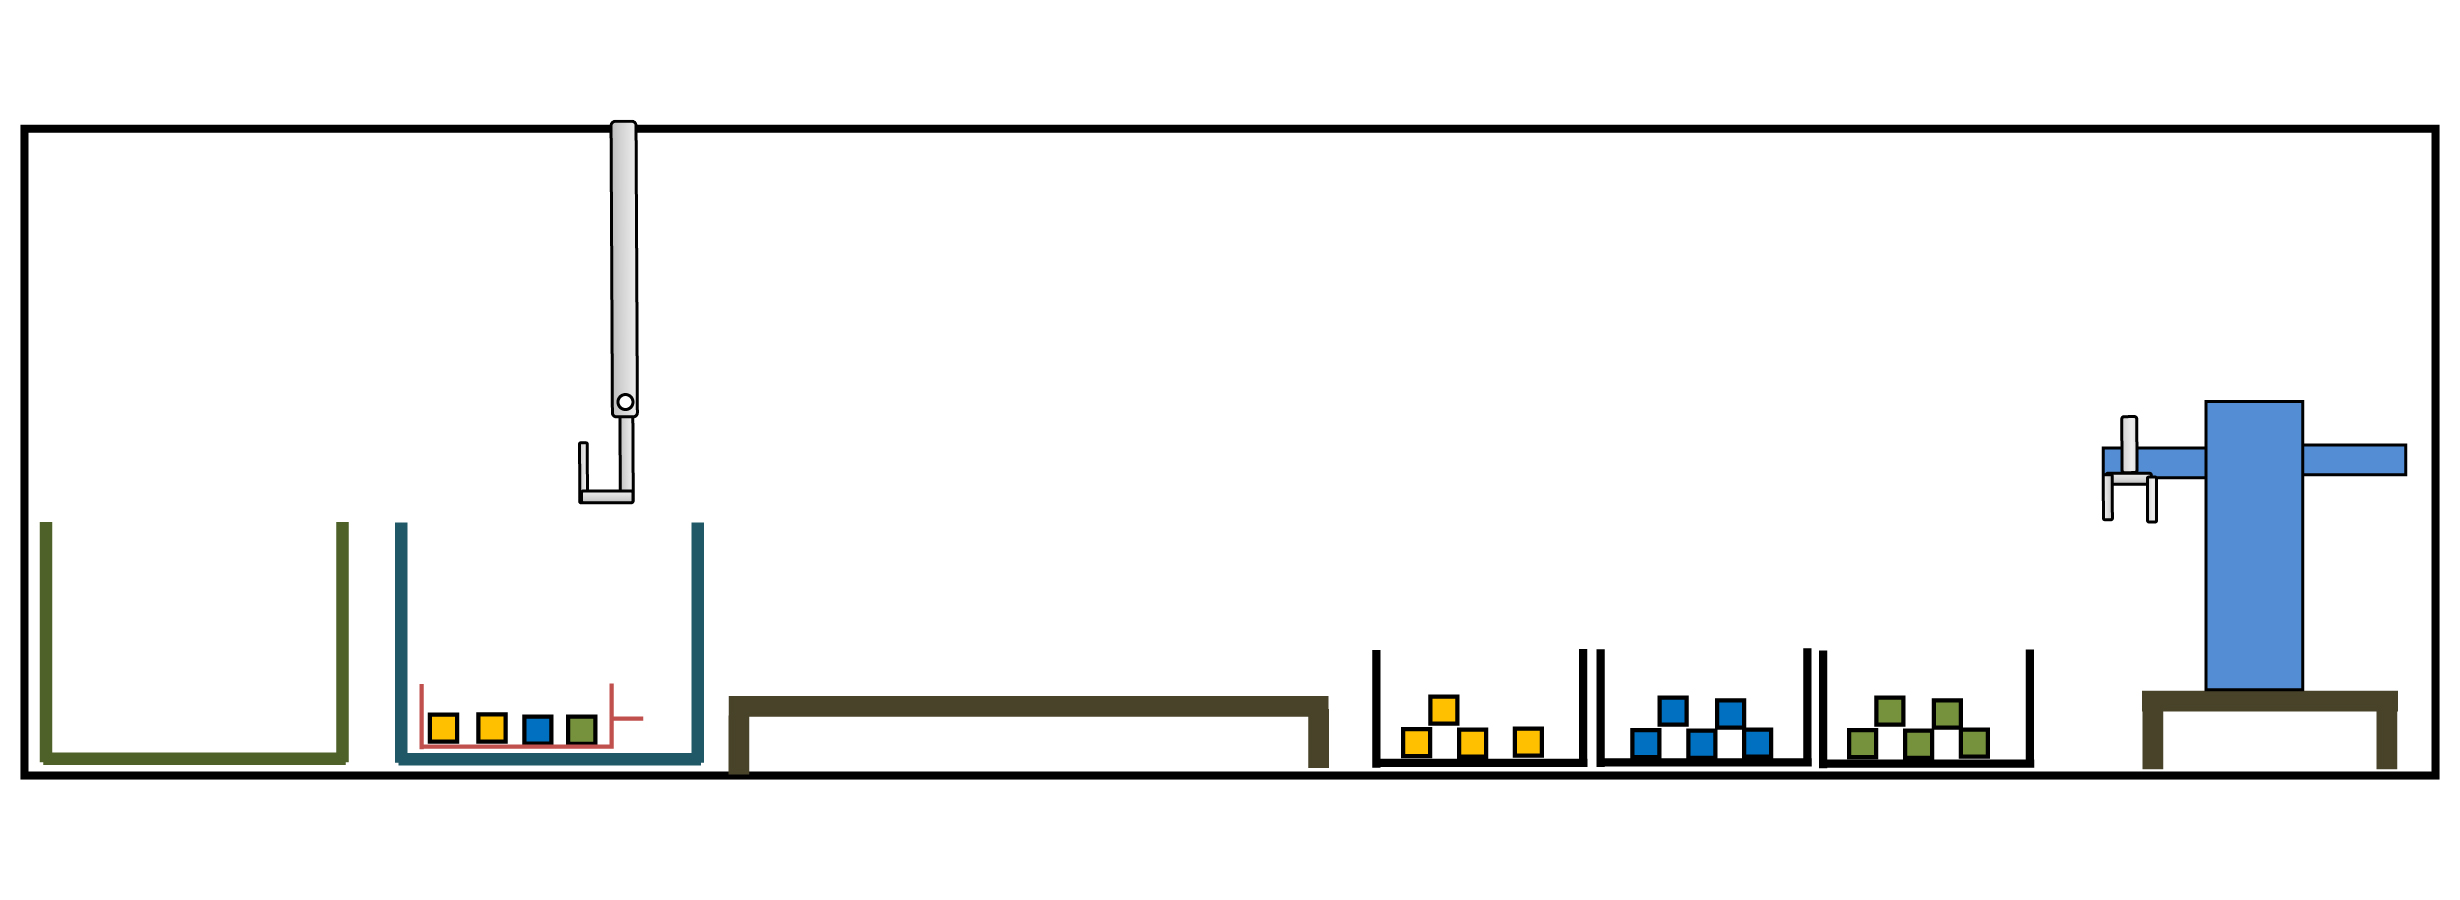
\includegraphics[width=14cm]{Figure/sfinal.jpg}
\caption{Goal state $S_G$.}
\label{fig:sf}
\end{figure}
Figure~\ref{fig:sf} depicts the goal state $S_G$ for the kitting workstation. The expression of the goal state in PDDL is described below.


\begin{itemize}
\item line 78: \texttt{:goal} is a keyword used to signal a planner about the goal state to reach. All the predicates and functions in the goal state must be true.
\item line 80--82: The quantity of parts of a specific type in \constsmall{kit\_a2b1c1} should match the capacity of parts of a specific type for \constsmall{kit\_a2b1c1}. The quantity of parts in \constsmall{kit\_a2b1c1} is increased in the operator \op{put-part}. The initial quantity of parts in \constsmall{kit\_a2b1c1} (lines 62--64) and its capacity (lines 58--60) are set in the initial state. Note that we are not specifying which instance of \class{Part} should go in \constsmall{kit\_a2b1c1} but rather the number of \class{Parts} of a specific type that \constsmall{kit\_a2b1c1} must have.
\item line 83: \constsmall{kit\_a2b1c1} should be placed in the large box with kits \constsmall{finished\_kit\_receiver}.
\end{itemize}

\subsection{Domain Independent Planning System}
From the domain and problem files, a domain independent planning system such as the forward-chaining partial-order planning system from Coles \textit{et al.}~\cite{Coles.ICAPS.2010} may be run to create a static plan file. This plan file contains a sequence of actions that will transition the system from the initial state to the goal state. In order to maintain flexibility, it is desired that detailed information that is subject to change should be ``late-bound'' to the plan. In other words, specific information is acquired directly before that information needs to be used by the system. This allows for last minute changes in this information. For example, the location of a kit tray on a work table may be different from run to run. However, one would like to be able to use the same planning sequence for constructing the kit independent of the tray's exact position.
To compensate for this lack of exact knowledge, the plans that are generated by the PDDL planning system contain only high-level actions.

The list below shows an example of a plan generated by a planner for the PDDL domain and problem files discussed previously in this document.

\begin{itemize}
\item $A1$:(\opsmall{attach-endeffector} \constsmall{robot\_1} \constsmall{tray\_gripper} \constsmall{tray\_gripper\_holder} \constsmall{changing\_station\_1})
\item $A2$:(\opsmall{take-kittray} \constsmall{robot\_1} \constsmall{kit\_tray\_1} \constsmall{empty\_kit\_tray\_supply} \constsmall{tray\_gripper} \constsmall{work\_table\_1})
\item $A3$:(\opsmall{put-kittray} \constsmall{robot\_1} \constsmall{kit\_tray\_1} \constsmall{work\_table\_1})
\item $A4$:(\opsmall{create-kit} \constsmall{kit\_a2b1c1} \constsmall{kit\_tray\_1} \constsmall{work\_table\_1})
\item $A5$:(\opsmall{remove-endeffector} \constsmall{robot\_1} \constsmall{tray\_gripper} \constsmall{tray\_gripper\_holder} \constsmall{changing\_station\_1})
\item $A6$:(\opsmall{attach-endeffector} \constsmall{robot\_1} \constsmall{part\_gripper} \constsmall{part\_gripper\_holder} \constsmall{changing\_station\_1})
\item $A7$:(\opsmall{look-for-part} \constsmall{robot\_1} \constsmall{part\_c\_1} \constsmall{part\_c\_tray} \constsmall{kit\_a2b1c1} \constsmall{work\_table\_1} \constsmall{part\_gripper})
\item $A8$:(\opsmall{take-part} \constsmall{robot\_1} \constsmall{part\_c\_1} \constsmall{part\_c\_tray} \constsmall{part\_gripper} \constsmall{work\_table\_1} \constsmall{kit\_a2b1c1})
\item $A9$:(\opsmall{put-part} \constsmall{robot\_1} \constsmall{part\_c\_1} \constsmall{kit\_a2b1c1} \constsmall{work\_table\_1} \constsmall{part\_c\_tray})
\item $A10$:(\opsmall{look-for-part} \constsmall{robot\_1} \constsmall{part\_b\_1} \constsmall{part\_b\_tray} \constsmall{kit\_a2b1c1} \constsmall{work\_table\_1} \constsmall{part\_gripper})
\item $A11$:(\opsmall{take-part} \constsmall{robot\_1} \constsmall{part\_b\_1} \constsmall{part\_b\_tray} \constsmall{part\_gripper} \constsmall{work\_table\_1} \constsmall{kit\_a2b1c1})
\item $A12$:(\opsmall{put-part} \constsmall{robot\_1} \constsmall{part\_b\_1} \constsmall{kit\_a2b1c1} \constsmall{work\_table\_1} \constsmall{part\_b\_tray})
\item $A13$:(\opsmall{look-for-part} \constsmall{robot\_1} \constsmall{part\_a\_2} \constsmall{part\_a\_tray} \constsmall{kit\_a2b2c1} \constsmall{work\_table\_1} \constsmall{part\_gripper})
\item $A14$:(\opsmall{take-part} \constsmall{robot\_1} \constsmall{part\_a\_2} \constsmall{part\_a\_tray} \constsmall{part\_gripper} \constsmall{work\_table\_1} \constsmall{kit\_a2b1c1})
\item $A15$:(\opsmall{put-part} \constsmall{robot\_1} \constsmall{part\_a\_2} \constsmall{kit\_a2b1c1} \constsmall{work\_table\_1} \constsmall{part\_a\_tray})
\item $A16$:(\opsmall{look-for-part} \constsmall{robot\_1} \constsmall{part\_a\_1} \constsmall{part\_a\_tray} \constsmall{kit\_a2b1c1} \constsmall{work\_table\_1} \constsmall{part\_gripper})
\item $A17$:(\opsmall{take-part} \constsmall{robot\_1} \constsmall{part\_a\_1} \constsmall{part\_a\_tray} \constsmall{part\_gripper} \constsmall{work\_table\_1} \constsmall{kit\_a2b1c1})
\item $A18$:(\opsmall{put-part} \constsmall{robot\_1} \constsmall{part\_a\_1} \constsmall{kit\_a2b1c1} \constsmall{work\_table\_1} \constsmall{part\_a\_tray})
\item $A19$:(\opsmall{remove-endeffector} \constsmall{robot\_1} \constsmall{part\_gripper} \constsmall{part\_gripper\_holder} \constsmall{changing\_station\_1})
\item $A20$:(\opsmall{attach-endeffector} \constsmall{robot\_1} \constsmall{tray\_gripper} \constsmall{tray\_gripper\_holder} \constsmall{changing\_station\_1})
\item $A21$:(\opsmall{take-kit} \constsmall{robot\_1} \constsmall{kit\_a2b1c1} \constsmall{work\_table\_1} \constsmall{tray\_gripper})
\item $A22$:(\opsmall{put-kit} \constsmall{robot\_1} \constsmall{kit\_a2b1c1} \constsmall{finished\_kit\_receiver})
\end{itemize}

\subsubsection{How to Install and Run the Planner}\label{section:planner}
This section describes the steps to install and run a planner on the PDDL domain and problem files in order to generate a plan. The planner described in this section uses a forward-chaining partial-order planning~\cite{Coles.ICAPS.2010}. We have chosen this planner because it has the ability to deal with numeric fluents.


%%%%%%%%%%%%%%%%%%%%%%% HOW TO -- Configure your Environment to Run the Planner %%%%%%%%%%%%%%%%%%%%%%%

\begin{table}[H]
\begin{tabular}{ll} % centered columns (4 columns)
\raisebox{-16 pt}{
\includegraphics[width=1.5cm]{Figure/gears2.png}} & \textbf{\textcolor{BrickRed}{HOW TO -- } Configure the Environment to Run the Planner}.  
\end{tabular}
\label{table:nonlin} % is used to refer this table in the text
\end{table}

To compile the planner, the following tools are required:
\begin{itemize}
\item[\textcolor{BrickRed}{$\blacksquare$}] \texttt{cmake}
\item[\textcolor{BrickRed}{$\blacksquare$}] The CBC mixed integer programming solver (\url{https://projects.coin-or.org/Cbc/})
\item[\textcolor{BrickRed}{$\blacksquare$}] \texttt{perl}, \texttt{bison} and \texttt{flex} to build the parser
\end{itemize}

These are packaged with most Linux distributions - on Ubuntu/Debian, the following should suffice:
\begin{itemize}
\item[\textcolor{BrickRed}{$\blacksquare$}] \texttt{sudo apt-get install cmake coinor-libcbc-dev coinor-libclp-dev \textbackslash \\coinor-libcoinutils-dev bison flex}
\end{itemize}

The CBC source code can be retrieved in two ways:

\begin{enumerate}
\item Local copy: \texttt{ipmas/planner/coin-Cbc.tar.gz}
\item SVN: \footnotesize{\texttt{svn co https://projects.coin-or.org/svn/Cbc/stable/2.8 coin-Cbc}}
\end{enumerate}

If CBC is retrieved using option 1, unzip \texttt{coin-Cbc.tar.gz} to generate the \texttt{coin-Cbc} directory.\\ 

Perform the following steps.
\begin{itemize}
\item[\textcolor{BrickRed}{$\blacksquare$}] \texttt{cd coin-Cbc}
\item[\textcolor{BrickRed}{$\blacksquare$}] \texttt{./configure -C}: Runs a configure script that generates the make file.
\item[\textcolor{BrickRed}{$\blacksquare$}] \texttt{make}: Builds the Cbc library and executable program.
\item[\textcolor{BrickRed}{$\blacksquare$}] \texttt{make test}: Builds and runs the Cbc unit test program.
\item[\textcolor{BrickRed}{$\blacksquare$}] \texttt{make install}: Installs libraries, executables and header files in directories \texttt{coin-Cbc/lib}, \texttt{coin-Cbc/bin} and \texttt{coin-Cbc/include}.
\end{itemize}

%%%%%%%%%%%%%%%%%%%%%%% HOW TO -- Install and Compile the Planner %%%%%%%%%%%%%%%%%%%%%%%

\begin{table}[H]
\begin{tabular}{ll} % centered columns (4 columns)
\raisebox{-16 pt}{
\includegraphics[width=1.5cm]{Figure/gears2.png}} & \textbf{\textcolor{BrickRed}{HOW TO -- } Install, Configure, and Compile the Planner}.  
\end{tabular}
\label{table:nonlin} % is used to refer this table in the text
\end{table}

The planner can be found at \texttt{ipmas/planner/popf2-11jun2011.tar.bz2}. Unzip \texttt{popf2-11jun2011.tar.bz2} to get the \texttt{tempo-sat-popf2} directory, then:
\begin{itemize}
\item[\textcolor{BrickRed}{$\blacksquare$}] cd \texttt{tempo-sat-popf2}
\item[\textcolor{BrickRed}{$\blacksquare$}] \texttt{./build}
\end{itemize}

New files and directories are created in the \texttt{tempo-sat-popf2/compile/} directory. However, the executable is not generated at this point and errors should be displayed. To fix this, open \texttt{tempo-sat-popf2/compile/CMakeCache.txt} in a text editor and edit the following lines. Note that \texttt{<path>} is the absolute path that leads to the \texttt{coin-Cbc} directory.


\begin{itemize}
\item[\textcolor{BrickRed}{$\blacksquare$}] \textbf{line 24}: \texttt{CBC\_INCLUDES:PATH=<path>/include}
\item[\textcolor{BrickRed}{$\blacksquare$}] \textbf{line 33}: \texttt{CGL\_INCLUDES:PATH=<path>/include}
\item[\textcolor{BrickRed}{$\blacksquare$}] \textbf{line 36}: \texttt{CGL\_LIBRARIES:FILEPATH=/usr/lib/libCgl.so.0}
\item[\textcolor{BrickRed}{$\blacksquare$}] \textbf{line 39}: \texttt{CLP\_INCLUDES:PATH=<path>/include}
\item[\textcolor{BrickRed}{$\blacksquare$}] \textbf{line 186}: \texttt{COINUTILS\_INCLUDES:PATH=<path>/include}
\item[\textcolor{BrickRed}{$\blacksquare$}] \textbf{line 230}: \texttt{OSICLP\_LIBRARIES:FILEPATH=/usr/lib/libOsiClp.so.0}
\item[\textcolor{BrickRed}{$\blacksquare$}] \textbf{line 233}: \texttt{OSI\_INCLUDES:PATH=<path>/include}
\item[\textcolor{BrickRed}{$\blacksquare$}] \textbf{line 236}: \texttt{OSI\_LIBRARIES:FILEPATH=/usr/lib/libOsi.so.0}
\end{itemize}

Recompile the planner:
\begin{itemize}
 \item[\textcolor{BrickRed}{$\blacksquare$}] \texttt{./build}
\end{itemize}




%%%%%%%%%%%%%%%%%%%%%%% HOW TO -- Install and Compile the Planner %%%%%%%%%%%%%%%%%%%%%%%

\begin{table}[H]
\begin{tabular}{ll} % centered columns (4 columns)
\raisebox{-16 pt}{
\includegraphics[width=1.5cm]{Figure/gears2.png}} & \textbf{\textcolor{BrickRed}{HOW TO -- } Run the Planner}.  
\end{tabular}
\label{table:nonlin} % is used to refer this table in the text
\end{table}
To run the planner, the path to the PDDL domain and problem files should be identified. The format of the PDDL files must be \texttt{.pddl}. The following command run the planner on the PDDL files.

\begin{itemize}
  \item[\textcolor{BrickRed}{$\blacksquare$}] \texttt{./plan <path-to-domain-file> <path-to-problem-file> <solution>}
    \begin{itemize}
      \item[\textcolor{BrickRed}{$\square$}] \texttt{<path-to-domain-file>}: Path to the domain file.
      \item[\textcolor{BrickRed}{$\square$}] \texttt{<path-to-problem-file>}: Path to the problem file.
      \item[\textcolor{BrickRed}{$\square$}] \texttt{<solution>}: Generated plan file.
    \end{itemize}
\end{itemize}


% \begin{figure}[h!]
%  \centering
%  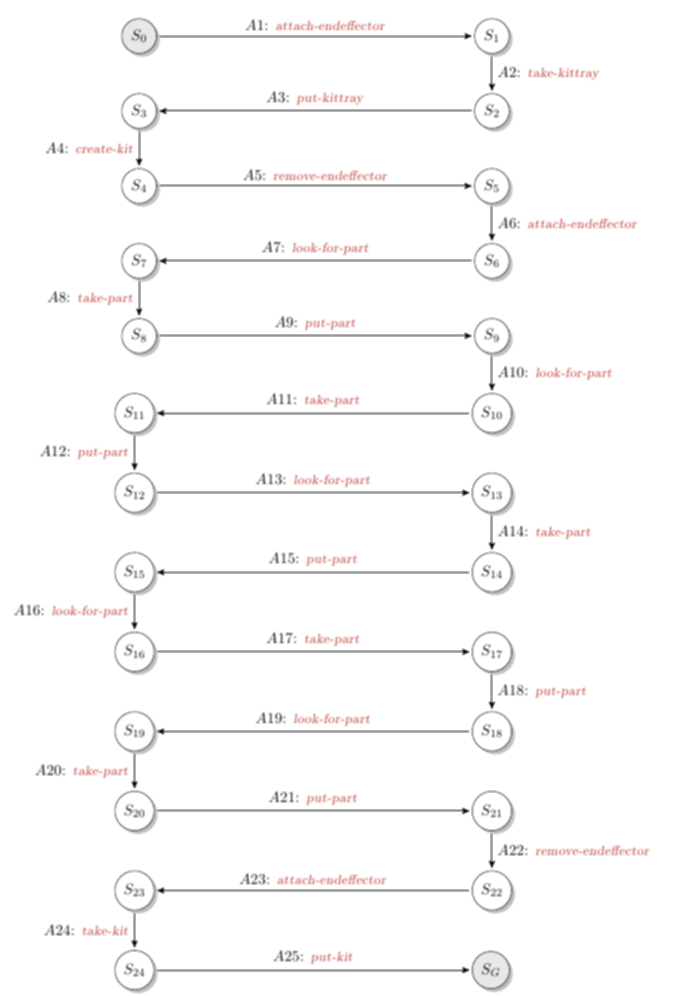
\includegraphics[width=8cm]{Figure/plan.jpg}
% \end{figure}

% \begin{figure}[h!]
%  \centering
% \scalebox{.5}{
% \begin{tikzpicture}[node distance=1.5cm, every edge/.style={link}]
% 
%   %%%%%%%%%%%%%%%%%%%%%%%%%%%%%%%%%%%%%%%%%%%%
%   %---------- Main
%   %%%%%%%%%%%%%%%%%%%%%%%%%%%%%%%%%%%%%%%%%%%%
%   \node[cloud2] (S0)  {$S_0$};
%   \node[cloud] (S1) [right=8cm of S0]{$S_1$};
%   \node[cloud] (S2) [below=1cm of S1]{$S_2$};
%   \node[cloud] (S3) [left=8cm of S2]{$S_3$};
%   \node[cloud] (S4) [below=1cm of S3]{$S_4$};
%   \node[cloud] (S5) [right=8cm of S4]{$S_5$};
%   \node[cloud] (S6) [below=1cm of S5]{$S_6$};
%   \node[cloud] (S7) [left=8cm of S6]{$S_7$};
%   \node[cloud] (S8) [below=1cm of S7]{$S_8$};
%   \node[cloud] (S9) [right=8cm of S8]{$S_9$};
%   \node[cloud] (S10) [below=1cm of S9]{$S_{10}$};
%   \node[cloud] (S11) [left=8cm of S10]{$S_{11}$};
%   \node[cloud] (S12) [below=1cm of S11]{$S_{12}$};
%   \node[cloud] (S13) [right=8cm of S12]{$S_{13}$};
%   \node[cloud] (S14) [below=1cm of S13]{$S_{14}$};
%   \node[cloud] (S15) [left=8cm of S14]{$S_{15}$};
%   \node[cloud] (S16) [below=1cm of S15]{$S_{16}$};
%   \node[cloud] (S17) [right=8cm of S16]{$S_{17}$};
%   \node[cloud] (S18) [below=1cm of S17]{$S_{18}$};
%   \node[cloud] (S19) [left=8cm of S18]{$S_{19}$};
%   \node[cloud] (S20) [below=1cm of S19]{$S_{20}$};
%   \node[cloud] (S21) [right=8cm of S20]{$S_{21}$};
%   \node[cloud] (S22) [below=1cm of S21]{$S_{22}$};
%   \node[cloud] (S23) [left=8cm of S22]{$S_{23}$};
%   \node[cloud] (S24) [below=1cm of S23]{$S_{24}$};
%   \node[cloud2] (SG) [right=8cm of S24]{$S_G$};
% 
% \draw[myarrow] (S0.east) -- node [above] {$A1$}(S1.west);
% \draw[myarrow] (S1.south) -- node [right] {$A2$}(S2.north);
% \draw[myarrow] (S2.west) --  node [above] {$A3$}(S3.east);
% \draw[myarrow] (S3.south) --  node [left] {$A4$}(S4.north);
% \draw[myarrow] (S4.east) --  node [above] {$A5$}(S5.west);
% \draw[myarrow] (S5.south) --  node [right] {$A6$}(S6.north);
% \draw[myarrow] (S6.west) --  node [above] {$A7$}(S7.east);
% \draw[myarrow] (S7.south) --  node [left] {$A8$}(S8.north);
% \draw[myarrow] (S8.east) --  node [above] {$A9$}(S9.west);
% \draw[myarrow] (S9.south) --  node [right] {$A10$}(S10.north);
% \draw[myarrow] (S10.west) --  node [above] {$A11$}(S11.east);
% \draw[myarrow] (S11.south) --  node [left] {$A12$}(S12.north);
% \draw[myarrow] (S12.east) --  node [above] {$A13$}(S13.west);
% \draw[myarrow] (S13.south) --  node [right] {$A14$}(S14.north);
% \draw[myarrow] (S14.west) --  node [above] {$A15$}(S15.east);
% \draw[myarrow] (S15.south) -- node [left] {$A16$}(S16.north);
% \draw[myarrow] (S16.east) -- node [above] {$A17$}(S17.west);
% \draw[myarrow] (S17.south) -- node [right] {$A18$}(S18.north);
% \draw[myarrow] (S18.west) -- node [above] {$A19$}(S19.east);
% \draw[myarrow] (S19.south) -- node [left] {$A20$}(S20.north);
% \draw[myarrow] (S20.east) -- node [above] {$A21$}(S21.west);
% \draw[myarrow] (S21.south) -- node [right] {$A22$}(S22.north);
% \draw[myarrow] (S22.west) -- node [above] {$A23$}(S23.east);
% \draw[myarrow] (S23.south) -- node [left] {$A24$}(S24.north);
% \draw[myarrow] (S24.east) -- node [above] {$A25$}(SG.west);
% 
% \end{tikzpicture}
% }
% \caption{Example of plan generated with the kitting domain and problem files.}
% \label{fig:plan}
% \end{figure} 

\subsection{MySQL Database}
While the knowledge representation presented in this document provides the \lq\lq{}slots\rq\rq{} necessary for representing dynamic information, the
static file structure makes the utilization of these slots awkward. It is desirable to be able to represent the dynamic information in a dynamic database.
For this reason, the authors have developed a technique for automatically generating tables for storing,  and access functions
for obtaining, the data from the ontology in a MySQL database.

Reading data from and to the MySQL database instead of the ontology file offers the community easy access to a live data structure. Furthermore, it is more practical to modify the information stored in a database than if it was stored in an ontology, which in some cases, requires the deletion and re-creation of the whole file. A literature review reveals many efforts and methodologies that have been designed to produce SQL databases from ontologies. Our effort builds upon the work of Astrova \textit{et al.}\cite{Astrova2007}.

In addition to generating and filling the database tables, the authors have created tools that automatically generate a set of {\cpp} classes for reading and writing
information to the kitting MySQL database. The choice of {\cpp} was a team preference and we believe that other object-oriented languages could have been used in this project.

The Generator tool is a graphical user interface developed in Java, allowing the user to store data from OWL files into a MySQL database. This tool also permits the user to query the database using the {\cpp} function calls. The tool Generator is composed of the following functionalities:
\begin{enumerate}
 \item Convert OWL documents into SQL syntax (OWL to SQL).
 \item Translate SQL syntax to OWL language in order to modify an OWL document (SQL to OWL).
 \item Convert the OWL language into {\cpp} classes (OWL to {\cpp}).
\end{enumerate}

To date, only steps 1. and 3. have been implemented and will be covered in this document. In order to generate the SQL database and {\cpp} classes, the OWL object model must be mapped to the {\cpp} object model and the relational SQL model.  To quote the OWL 2 Web Ontology website~\cite{OWLspec}, ``Entities are the fundamental building blocks of OWL 2 ontologies, 
and they define the vocabulary --the named terms-- of an ontology. In logic, the set of entities is usually said to constitute the 
signature of an ontology''. Therefore, the notions of single-valued and multi-valued properties as well as the inheritance must be 
mapped from the ontology to the SQL database and {\cpp} classes. The mapping from OWL proceeds as follows:
\begin{itemize}
\item Data properties: In an ontology, data properties link an individual to a data value. Single-valued data properties are mapped into a SQL table entry or {\cpp} class
variable with the corresponding type of the original property. For example, in the ontology a robot has a single-valued data 
property \texttt{hasRobot\_Description}, represented in the
SQL database as a \texttt{varchar} and in the corresponding {\cpp} class as \texttt{std:string}. 
Multi-valued data properties are mapped from the ontology into the SQL database as a table and into the {\cpp} class as a \texttt{std:vector} with the corresponding
type of the original property. For example,
in the ontology a stock keeping unit has a multi-valued
data property \texttt{hasSku\_EndEffectorRefs}. This maps to a SQL table containing \texttt{varchar} entries and the {\cpp}
\texttt{std::vector\textless std::string\textgreater} in the corresponding {\cpp} class.

\item Object property: In an ontology, object properties link one individual to another individual. 
The single-valued object properties are mapped to a SQL table entry or {\cpp} class
variable. Their type is a pointer to the range of the object properties. For example, in the ontology a solid object has the object property \texttt{hasRobot\_Description} 
linking it to a physical location. In the SQL database, we use a foreign key to link the two entries. In the {\cpp} classes, this is represented by a reference to a physical location: \texttt{PhysicalLocation* hasSolidObject\_PrimaryLocation}.
Multi-valued object properties are mapped from the ontology into the SQL database as a table and into the {\cpp} class as a \texttt{std:vector} of pointers referencing objects of the range of the property.  For example, a solid object also has a list of secondary locations corresponding to a multi-valued object property in the ontology: {\scriptsize\texttt{std::vector\\ \textless PhysicalLocation*\textgreater hasSolidObject\_SecondaryLocation}}.
\end{itemize}

\subsubsection{MySQL Database Generation}\label{ss:ontology2db}
\begin{figure}[h!t!]
\centering
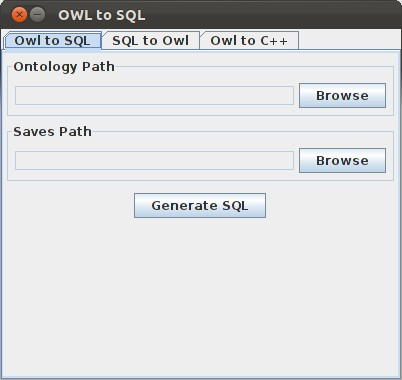
\includegraphics[width=9cm]{Figure/OWLtoSQL001.jpeg}
\caption{Owl to SQL tab.}
\label{fig:owl2sqlx}
\end{figure}



This section provides basic information on the Generator Java tool. Specific information on the tool\rq{}s usage is included in the tool\rq{}s manual.
Converting an OWL ontology to SQL script files is easily performed using the \texttt{Owl to SQL} tab  (see Figure~\ref{fig:owl2sqlx}). 

%%%%%%%%%%%%%%%%%%%%%%% HOW TO %%%%%%%%%%%%%%%%%%%%%%%

\begin{table}[H]
\begin{tabular}{ll} % centered columns (4 columns)
\raisebox{-16 pt}{
\includegraphics[width=1.5cm]{Figure/gears2.png}} & \textbf{\textcolor{BrickRed}{HOW TO -- } Set up your environment to run the Generator}.  
\end{tabular}
\label{table:nonlin} % is used to refer this table in the text
\end{table}

\begin{itemize}
  \item[\textcolor{BrickRed}{$\blacksquare$}] Install the Java Runtime Environment
    \begin{itemize}
      \item[\textcolor{BrickRed}{$\square$}] The Generator tool comes as a jar file. As such, the Java Runtime Environment should be installed on your system. This application can be found at \url{www.oracle.com}.
    \end{itemize}
  \item[\textcolor{BrickRed}{$\blacksquare$}] Install the MySQL Server and Client
    \begin{itemize}
      \item[\textcolor{BrickRed}{$\square$}] \textit{sudo apt-get update} (Update the package management tools)
      \item[\textcolor{BrickRed}{$\square$}] \textit{sudo apt-get dist-upgrade} (Install the latest software)
      \item[\textcolor{BrickRed}{$\square$}] \textit{sudo apt-get install mysql-server mysql-client} (Install the MySQL server and client packages). You will be asked to enter a password.
    \end{itemize}
\end{itemize}

You have now a MySQL database ready to run. Finally, we need the plugin \texttt{libmysqlcppconn-dev} which allows {\cpp} to connect to MySQL databases. It can be installed as follows:
\begin{itemize}
 \item[\textcolor{BrickRed}{$\blacksquare$}] \textit{sudo apt-get install libmysqlcppconn-dev}
\end{itemize}


%%%%%%%%%%%%%%%%%%%%%%% HOW TO -- Run the Generator %%%%%%%%%%%%%%%%%%%%%%%

\begin{table}[H]
\begin{tabular}{ll} % centered columns (4 columns)
\raisebox{-16 pt}{
\includegraphics[width=1.5cm]{Figure/gears2.png}} & \textbf{\textcolor{BrickRed}{HOW TO -- } Run the Generator}.  
\end{tabular}
\label{table:nonlin} % is used to refer this table in the text
\end{table}

The Generator tool can be launched using either one of these two following methods:
\begin{enumerate}
 \item \textit{java -jar Generator.jar}
 \item Right-click on Generator.jar and select the option ``Open With OpenJDK Java 6 Runtime". Note that this message will be different for future releases of the Java Runtime Environment.
\end{enumerate}


%%%%%%%%%%%%%%%%%%%%%%% HOW TO -- Create SQL files %%%%%%%%%%%%%%%%%%%%%%%

\begin{table}[H]
\begin{tabular}{ll} % centered columns (4 columns)
\raisebox{-16 pt}{
\includegraphics[width=1.5cm]{Figure/gears2.png}} & \textbf{\textcolor{BrickRed}{HOW TO -- }Create SQL files}.  
\end{tabular}
\label{table:nonlin} % is used to refer this table in the text
\end{table}

\begin{enumerate}
  \item Run the Generator (see previous \textcolor{BrickRed}{HOW TO}).
  \item Choose the \texttt{Owl to SQL} tab.
    \begin{itemize}
      \item[\textcolor{BrickRed}{$\blacksquare$}] Ontology Path: The OWL file to be converted. Note that all \texttt{Import} statements in this file must use absolute paths.
      \item[\textcolor{BrickRed}{$\blacksquare$}] Saves Path: The directory where you want to save the SQL files.
    \end{itemize}
  \item Click the ``Generate SQL'' button to generate the SQL script files. Two files will be created by the tool:
    \begin{itemize}
      \item[\textcolor{BrickRed}{$\blacksquare$}] The file used to create tables in the database: \texttt{<inputfile>.owlCreateTable.sql} 
      \item[\textcolor{BrickRed}{$\blacksquare$}] The file used to populate the database tables: \texttt{<inputfile>.owlInsertInto.sql}. 
    \end{itemize}
\end{enumerate}

%%%%%%%%%%%%%%%%%%%%%%% HOW TO %%%%%%%%%%%%%%%%%%%%%%%

\begin{table}[H]
\begin{tabular}{ll} % centered columns (4 columns)
\raisebox{-16 pt}{
\includegraphics[width=1.5cm]{Figure/gears2.png}} & \textbf{\textcolor{BrickRed}{HOW TO -- }Create a MySQL Database and Fill the Tables}.  
\end{tabular}
\label{table:nonlin} % is used to refer this table in the text
\end{table}

\begin{itemize}
\item[\textcolor{BrickRed}{$\blacksquare$}] Connect to mysql. 
\begin{itemize}
 \item[\textcolor{BrickRed}{$\square$}] \textit{mysql -u root -p}: Enter the same password you used when you installed the MySQL server and client. You should be in the mysql shell if this succeeded (\textit{mysql>}).
\end{itemize}

\item[\textcolor{BrickRed}{$\blacksquare$}] Create a database:
  \begin{itemize}
    \item[\textcolor{BrickRed}{$\square$}] \texttt{mysql>} \textit{CREATE DATABASE OWL;}
      \begin{itemize}
	\item[\textcolor{BrickRed}{$\triangleright$}] \textit{OWL} is the name of the database (you can use a name of your choice).
      \end{itemize}
    \item[\textcolor{BrickRed}{$\square$}] Before performing the following commands, we need to tell MySQL which database we are planning to work with (\textit{OWL} in our case). This is done using:
      \begin{itemize}
	\item[\textcolor{BrickRed}{$\triangleright$}] \texttt{mysql>} \textit{USE OWL}
      \end{itemize}
  \end{itemize}
\item[\textcolor{BrickRed}{$\blacksquare$}] Create tables in the \textit{OWL} database:
\begin{itemize}
 \item[\textcolor{BrickRed}{$\square$}] \texttt{mysql>} \textit{source} \texttt{<path>/kittingInstances.owlCreateTable.sql};
\end{itemize}

\item[\textcolor{BrickRed}{$\blacksquare$}] Fill the tables:
\begin{itemize}
 \item[\textcolor{BrickRed}{$\square$}] \texttt{mysql>} \textit{source} \texttt{<path>/<inputfile>.owlInsertInto.sql};
\end{itemize}
\end{itemize}

\textcolor{BrickRed}{Note}: \texttt{<path>} designs the absolute path to the appropriate file.

\subsubsection{{\cpp} Class Generation and Usage}
As previously mentioned, the {\cpp} classes are automatically generated by the Generator tool. In addition to the class structure, 
Data Access Objects (DAO) that are needed to interact with the MySQL database are generated. 
To map the MySQL database and indirectly the ontology to {\cpp} classes, both the {\cpp} classes and
the DAO must be generated.

The {\cpp} class files (.cpp) and header files (.h) are generated in a two step process.
The first step does not depend on the content of the ontology, it only initializes the specific objects related to the MySQL connector driver
(see Figure~\ref{fig:headerclass}).

The second step generates all the {\cpp} headers and class files relative to our ontology. 
All of the \texttt{include} statements  are made directly in the {\cpp} class files, and only forward declarations are performed in the headers. 
This resolves problems associated with circular includes or multiple includes. All of the classes include the following methods:
\begin{itemize}
\item \texttt{get<private field>} - Method for getting a private field.
\item \texttt{set<private field>} - Method for setting a private field.
\item \texttt{explode} - Method that splits a string into a vector around matches of a given regular expression. 
\item \texttt{copy} -  Method that takes a {\cpp} map as input and copies the values from the map into the instance.
\item \texttt{get} - Method that reads data from the MySQL database.
\item \texttt{set} - Method that writes data to the MySQL database.
\end{itemize}

\begin{figure}[t!h!]
\begin{minipage}{.5\paperwidth}
\begin{mylisting}
\begin{Verbatim}[commandchars=\\\{\},fontsize=\scriptsize, numbersep=2pt]
\textbf{#ifndef} PARTSBIN_H_
\textbf{#define} PARTSBIN_H_
\textbf{#include} <cstdlib>
\textbf{#include} <iostream>
\textbf{#include} <map>
\textbf{#include} <string>
\textbf{#include} <vector>
\textbf{#include} <sstream>

\textbf{#include} "BoxyObject.h"
\textbf{class} DAO;
\textbf{class} PartsBin: \textbf{public} BoxyObject \{
    \textbf{private}:
        std::string hasBin_PartQuantity;
        std::string hasBin_PartSkuRef;
        \textbf{int} PartsBinID;
        DAO* dao;
    \textbf{public}:
        PartsBin(std::string name);
        ~PartsBin();
        \textbf{void} get(\textbf{int} id);
        \textbf{void} get(std::string name);
        \textbf{void} set(\textbf{int} id, PartsBin* obj);
        \textbf{void} set(std::string name);
        std::string gethasBin_PartQuantity();
        \textbf{void} sethasBin_PartQuantity(
            std::string _hasBin_PartQuantity);
        std::string gethasBin_PartSkuRef();
        \textbf{void} sethasBin_PartSkuRef(
            std::string _hasBin_PartSkuRef);
        \textbf{int} getPartsBinID();
        DAO* getdao();
        \textbf{void} setdao(DAO* _dao);
        \textbf{void} copy(std::map<std::string,
            std::string> object);
        std::vector<std::string> Explode(
            \textbf{const} std::string & str, \textbf{char} separator);
\};
\textbf{#endif} /* PARTSBIN_H_ */
\end{Verbatim}
\end{mylisting}
\end{minipage}
\caption{Header of a generated class.}
\label{fig:headerclass}
\end{figure}

The actual data access is provided through the use of a data access object (DAO).
DAOs provide an abstract interface to some type of database or other persistence
mechanism. DAOs map application calls to the database or persistence mechanism, 
thus providing some specific data operations without exposing
details of the database. The use of the DAO separates the data accesses that the application needs from how these needs can be satisfied with a specific
Database Management System (DBMS), database schema, etc. 
The different methods of the DAO are the same for any ontology. 
The concern here is not about the data, but only about the way to retrieve or store it. Only the four vectors filled by the
private \texttt{fillGetSqlQueries} method differ from one 
auto-generated {\cpp} file to another.

\begin{figure}[t!h!]
\begin{minipage}{.45\paperwidth}
\begin{mylisting}
\begin{Verbatim}[commandchars=\\\{\},fontsize=\footnotesize, numbers=left, numbersep=2pt]
\textbf{#ifndef} DAO_H_
\textbf{#define} DAO_H_
\textbf{#include} <cstdlib>
\textbf{#include} <iostream>
\textbf{#include} <map>
\textbf{#include} <vector>
\textbf{#include} <sstream>

\textbf{#include} "Connection.h"
\textbf{class} DAO \{
    \textbf{private}:
      std::vector<std::string> className;
      Connection* connection;
      std::vector<std::string> nameDone;
      std::map<std::string, std::string> map;
      std::string path; std::string pathmulti;
      \textbf{static} std::map<std::string, std::string>
        getSqlQueriesDataSingle;
      \textbf{static} std::map<std::string, 
			std::vector<std::string>>
			getSqlQueriesDataMulti;
      \textbf{static} std::map<std::string, 
			std::vector<std::string>>
			getSqlQueriesObjectSingle;
      \textbf{static} std::map<std::string, 
			std::vector<std::string>>
			getSqlQueriesObjectMulti;
      \textbf{static} std::map<std::string, 
			std::vector<std::string>>
			setSqlQueries;
      \textbf{static} std::map<std::string, 
			std::vector<std::string>>
			updateSqlQueries;
      \textbf{void} fillGetSqlQueries();
    \textbf{public}:
      DAO(std::string name); ~DAO();
      std::vector<std::string> getclassName();
      \textbf{void} setclassName(
		std::vector<std::string> _className);
      Connection* getconnection();
      \textbf{void} setconnection(Connection* _connection);
      std::map<std::string,std::string> 
      	get(std::string name);
      \textbf{void} set(std::map<std::string, std::string> data);
      std::vector<std::string> Explode(
		\textbf{const} std::string & str,
      \textbf{char separator});
\};
\textbf{#endif} /* DAO_H_ */
\end{Verbatim}
\end{mylisting}
\end{minipage}
\caption{Header of the DAO class.}
\label{fig:headerdao}
\end{figure}

When the DAO is generated, four vectors are built as follows (shown in Figure \ref{fig:headerdao}):

\begin{itemize}
\item line 17: A structure with the SQL query to select the characteristics of an entity. The table
relative to the entity itself and the ones relative to its super classes are queried.
\item line 18: A structure with the SQL query to select multi-valued attributes (multi-valued data) for a given entity.
\item line 19: A structure with the names of the tables linked to this entity in the ontology.
\item line 20: A structure with the names of the association tables linked to an object.
\end{itemize}

With these four structures, one is able to read (\texttt{get} method) and write (\texttt{set} method) data from and to the MySQL database. The \texttt{get} method fills 
a {\cpp} map and gets the object itself while the \texttt{copy} method handles the data. The \texttt{set} method is called with a {\cpp} map containing the values of the 
different attributes as input and writes these values into the MySQL database.



\begin{table}[!h!]
\begin{tabular}{ll} % centered columns (4 columns)
\raisebox{-16 pt}{
\includegraphics[width=1.5cm]{Figure/gears2.png}} & \textbf{\textcolor{BrickRed}{HOW TO -- }Generate {\cpp} Files}.  
\end{tabular}
\label{table:nonlin} % is used to refer this table in the text
%\caption[HOW TO -- Generate {\cpp} Files]
\end{table}

\begin{figure}[h!t!]
\centering
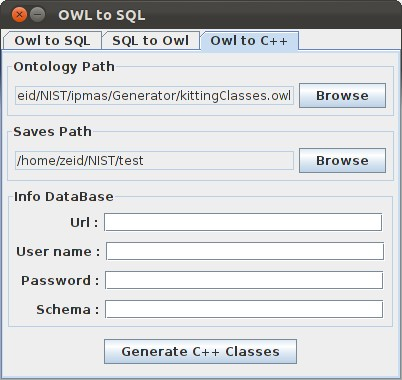
\includegraphics[width=8cm]{Figure/OWL2C++.jpeg}
\caption{Owl to C++ tab.}
\label{fig:owl2Cpp}
\end{figure}

\begin{enumerate}
  \item Run the Generator.
  \item Choose the \texttt{Owl to {\cpp}} tab (see Figure~\ref{fig:owl2Cpp}).
    \begin{itemize}
      \item[\textcolor{BrickRed}{$\blacksquare$}] Ontology Path: Path to the ontology classes (\texttt{kittingClasses.owl} in our example).
      \item[\textcolor{BrickRed}{$\blacksquare$}] Saves Path: The directory where you want to save the {\cpp} files.
      \item[\textcolor{BrickRed}{$\blacksquare$}] Url: The IP address of the machine hosting the database (127.0.0.1 if local).
      \item[\textcolor{BrickRed}{$\blacksquare$}] User name: User name used to connect to the MySQL database.
      \item[\textcolor{BrickRed}{$\blacksquare$}] Password: Password associated to the user name to connect to the MySQL database.
      \item[\textcolor{BrickRed}{$\blacksquare$}] Schema: This is the name of the database (\textit{OWL} in our example).
    \end{itemize}
\end{enumerate}

\subsubsection{Using the {\cpp} Classes to Access Data from the MySQL Database}

\begin{figure}[t!h!]
\begin{minipage}{.50\paperwidth}
\begin{mylisting}
\begin{Verbatim}[commandchars=\\\{\},fontsize=\footnotesize, numbers=left, numbersep=2pt]
#include "Point.h"
#include "PoseLocation.h"
#include "Vector.h"
#include "KitTray.h"

void CanonicalRobotCommand::
 getKitTrayLocation(string kit_tray_name)\{

  KitTray* kit_tray = \textbf{new} KitTray(kit_tray_name);
  kit_tray->get(kit_tray_name);

  PoseLocation* kit_tray_pose = \textbf{new} PoseLocation(
  kit_tray->gethasSolidObject_PrimaryLocation()->
 		getname());
  kit_tray_pose->get(kit_tray_pose->getname());

  //--Retrieve hasPoseLocation_Point
  Point * kit_tray_point =
  kit_tray_pose->gethasPoseLocation_Point();

  //--Retrieve hasPoseLocation_XAxis
  Vector * kit_tray_x_axis  =
  kit_tray_pose->gethasPoseLocation_XAxis();

  //--Retrieve hasPoseLocation_ZAxis
  Vector * kit_tray_z_axis  =
  kit_tray_pose->gethasPoseLocation_ZAxis();
\}
\end{Verbatim}
\end{mylisting}
\end{minipage}
\caption{Example using the generated {\cpp} classes.}
\label{fig:exampleofuse}
\end{figure}


Figure~\ref{fig:exampleofuse} depicts an example using the generated classes to retrieve the location of the kit tray \texttt{kit\_tray\_name} from the MySQL database. The different sections of the example are described below:

\begin{itemize}
\item lines 1--4: Include the different headers necessary to query MySQL tables. Here, the tables Point, PoseLocation, Vector, and KitTray are required.
\item line 9: Initialize an object from the class \texttt{KitTray} by passing its name.
\item line 10: Allow access to any data from the table KitTray.
\item lines 12--13: Initialize an object of type \texttt{PoseLocation} and allow access to any data from the table PoseLocation.
\item lines 18--19: Retrieve X, Y, and Z coordinates from the table Point for the kit tray \texttt{kit\_tray\_name}.
\item lines 22--23: Retrieve the X axis vector ($X_i$, $X_j$, $X_k$) from the table Vector for the kit tray \texttt{kit\_tray\_name}.
\item lines 26--27: Retrieve the Y axis vector ($Y_i$, $Y_j$, $Y_k$) from the table Vector for the kit tray \texttt{kit\_tray\_name}.
\end{itemize}
